% ─────────────────────────────────────────────────────────────
\subsection{Experimental Setup and Evaluation Methodology}
% ─────────────────────────────────────────────────────────────

All experiments were conducted on an AMD Ryzen~7 7435HS processor (3.10\,GHz, 16 logical cores).
Three datasets were used: (i)~the team-collected \textbf{Algiers} dataset (59 real landmarks,
multiple time windows); (ii)~\textbf{Solomon-50}~\cite{solomon50}, 50-node TOPTW benchmark
instances (\texttt{c/r/rc\_100\_50}) covering clustered, random, and mixed layouts; and
(iii)~\textbf{Solomon-100}~\cite{solomon100}, the full 100-node instances used for scalability
stress-testing. CPLEX was excluded from Solomon-100 due to prohibitive runtime and capped at
\textbf{30\,s} on Algiers.

The evaluated solvers are: \textsc{Greedy} (score- and ratio-priority variants),
\textsc{SA-Boltzmann}, \textsc{SA-Cauchy}, \textsc{Tabu}, \textsc{Tabu-Random}, \textsc{GRASP},
\textsc{Genetic-Tailored}, \textsc{Genetic-Score}, and \textsc{CPLEX}.
Stochastic solvers ran \textbf{5 times per instance} (25 runs over 5 instances); deterministic
solvers once. A multiprocessing framework with adaptive serialisation was used throughout.

\paragraph{Performance Metrics.}
\begin{itemize}[leftmargin=*, noitemsep, topsep=2pt]
  \item \textbf{Score}: total collected interest along the tour.
  \item \textbf{Optimality gap} (\%):
        $\mathrm{Gap} = \max\!\bigl(0,\;\tfrac{\text{Optimal}-\text{Score}}{\text{Optimal}}\times100\bigr)$,
        with CPLEX as ground truth for Solomon-50~\cite{solomon50} and
        Righini \& Salani~\cite{righini_salani} optima for Solomon-100~\cite{solomon100}.
  \item \textbf{Execution time} (s): wall-clock time per run.
  \item \textbf{Optimal-finding rate}: fraction of stochastic runs matching the known optimum.
\end{itemize}

\noindent\textsc{Genetic-Score} is excluded from optimality comparisons as its unconstrained
fitness generates infeasible tours; it is discussed in Section~\ref{sec:insights}.

% ─────────────────────────────────────────────────────────────
\subsection{Algiers Dataset}
% ─────────────────────────────────────────────────────────────

\begin{figure}[htbp]
  \centering
  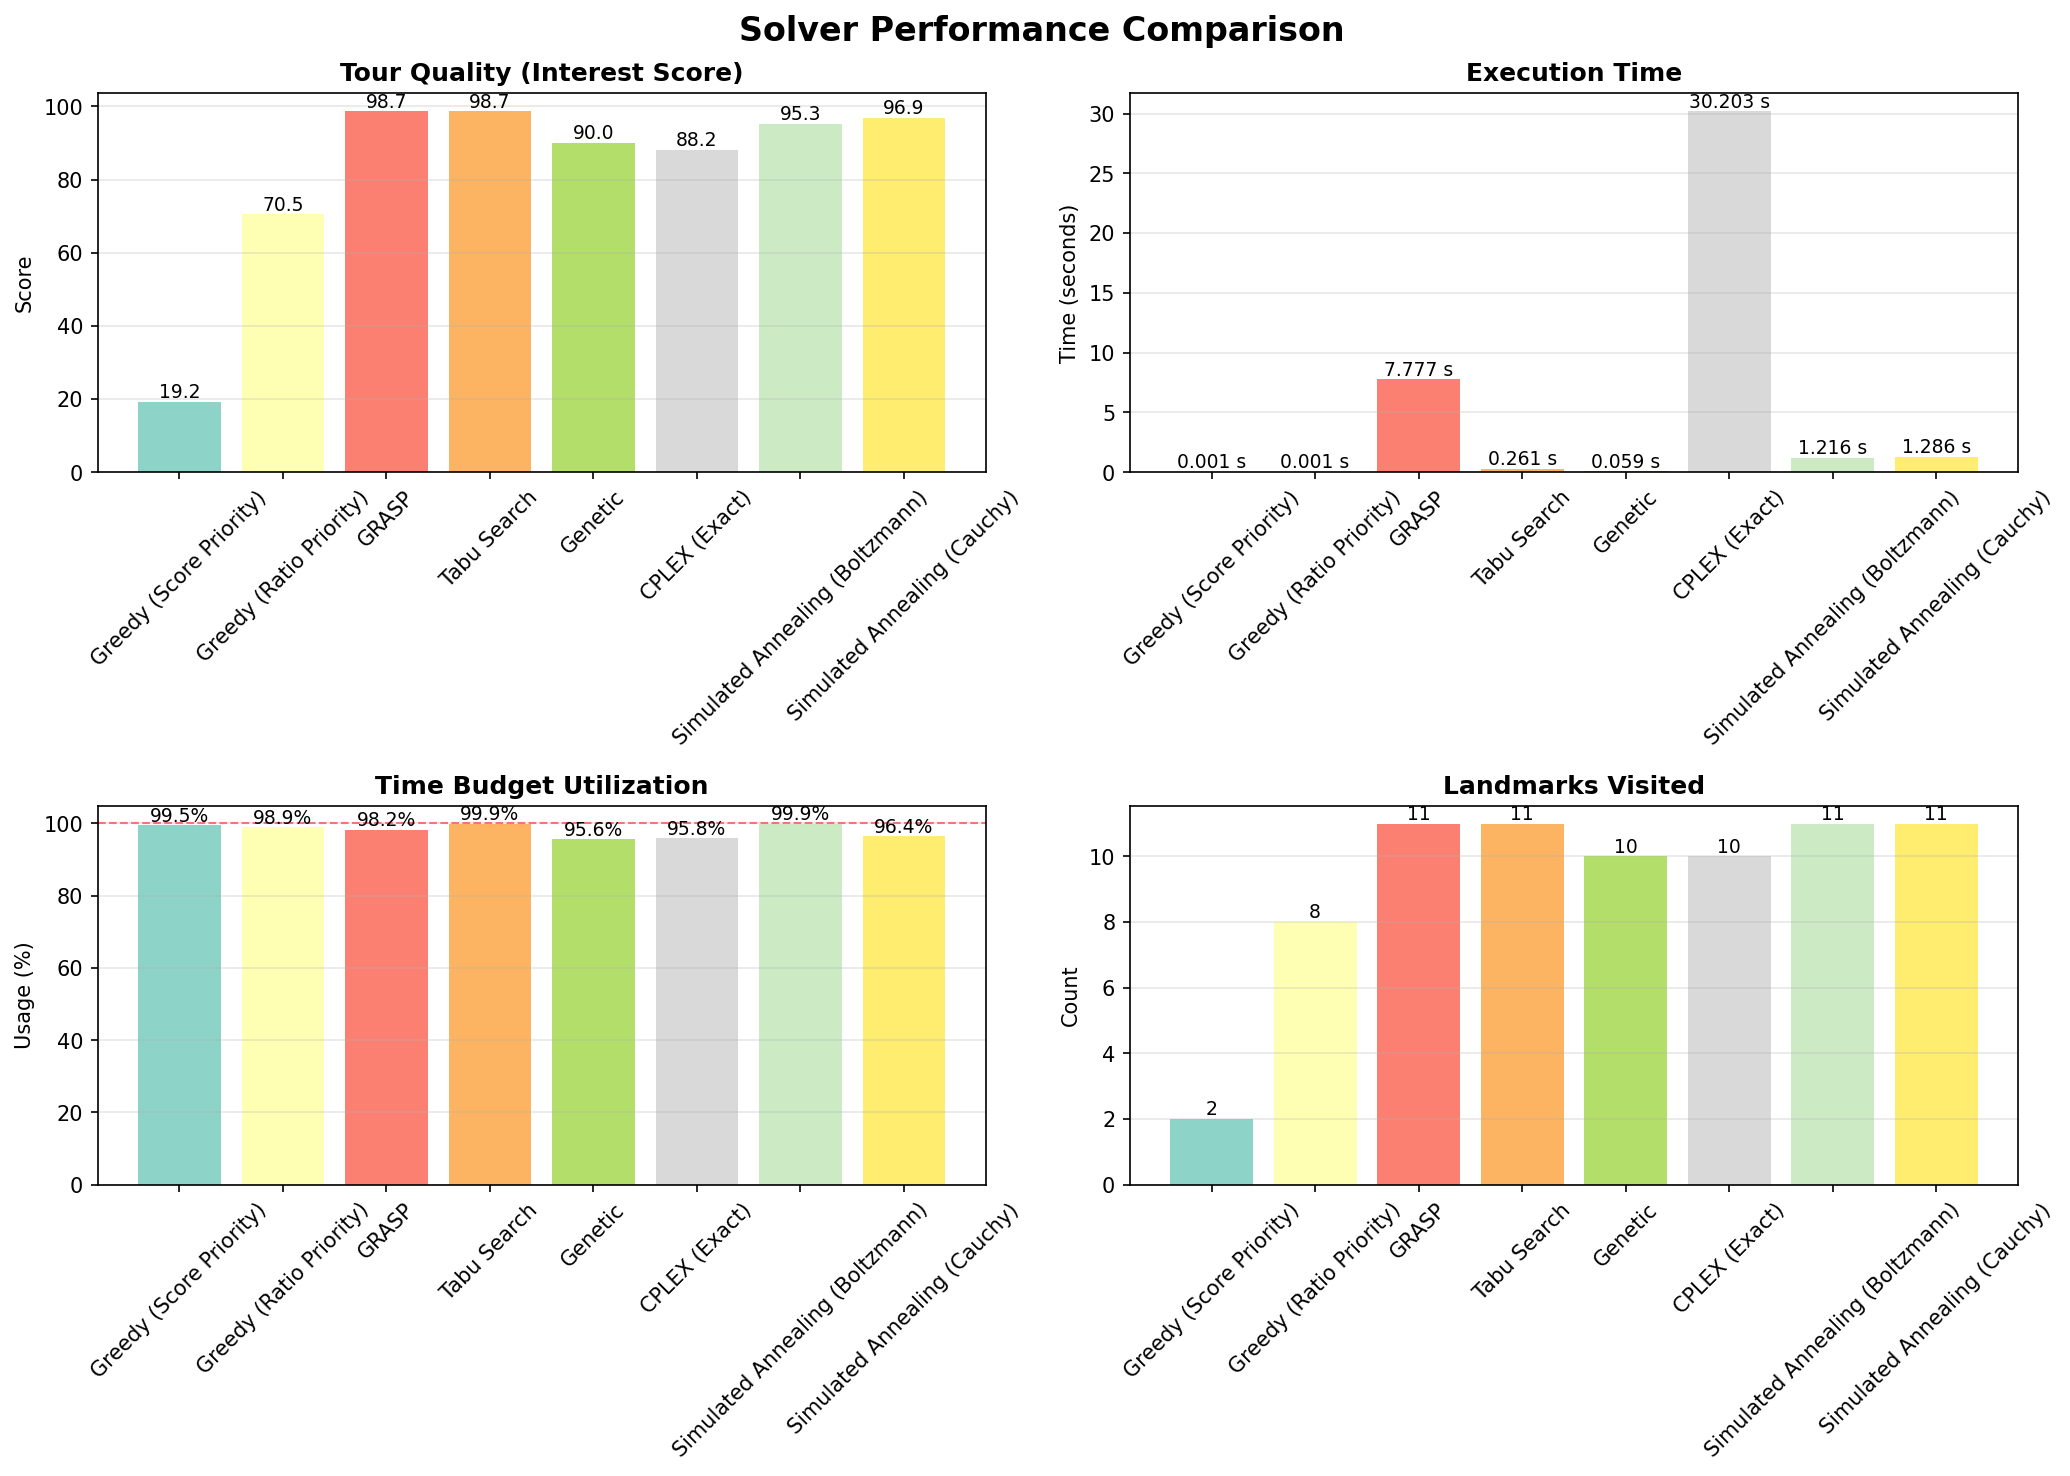
\includegraphics[width=\linewidth]{plots/Algiers_dataset_comparaison.png}
  \caption{Solver performance on the Algiers real-world dataset (59 landmarks): tour quality
           (interest score), execution time, time-budget utilisation, and landmarks visited.}
  \label{fig:algiers}
\end{figure}

Figure~\ref{fig:algiers} presents four performance views on the Algiers dataset.
\textsc{GRASP} and \textsc{Tabu} both attain the highest score of \textbf{98.7}
(11 landmarks, 98.2\% and 99.9\% budget utilisation);however \textsc{Tabu} attains the highest score
under only  0.261\,s the best speed–quality trade-off on this dataset.
 \textsc{SA-Cauchy} (96.9) and \textsc{SA-Boltzmann} (95.3) follow closely. \textsc{Genetic-Tailored} achieves 90.0 across 11 landmarks
in only 0.059\,s---. The \textsc{Greedy}
variants diverge sharply: Ratio-Priority scores 70.5 (8 landmarks) while Score-Priority
collapses to 19.2 (2 landmarks), confirming that score-greedy construction fails without
feasibility enforcement.

Despite being an exact solver, \textsc{CPLEX} reaches only 88.2 under its 30\,s cap---
insufficient to prove optimality on a 59-node instance with heterogeneous time windows.
\textsc{Tabu} (98.7 at 0.216\,s) and all top metaheuristics surpass it, illustrating the
practical advantage of local-search methods under strict time budgets.

% ─────────────────────────────────────────────────────────────
\subsection{Solomon-50: Solution Quality}
% ─────────────────────────────────────────────────────────────

\begin{figure}[htbp]
  \centering
  \begin{minipage}[t]{0.49\linewidth}
    \centering
    
\includegraphics[width=\linewidth]{plots/solomon50_scores.png}
    \caption{Score distributions on Solomon-50~\cite{solomon50} (box plot over 25 stochastic / 5 deterministic runs).}
    \label{fig:s50-scores}
  \end{minipage}\hfill
  \begin{minipage}[t]{0.49\linewidth}
    \centering
    
\includegraphics[width=\linewidth]{plots/solomon50_optimality.png}
    \caption{Optimality gap on Solomon-50~\cite{solomon50} (CPLEX-terminated instances only).}
    \label{fig:s50-opt}
  \end{minipage}
\end{figure}

\begin{figure}[htbp]
  \centering
  \begin{minipage}[t]{0.49\linewidth}
    \centering
    
\includegraphics[width=\linewidth]{plots/solomon50_times.png}
    \caption{Mean execution time per solver on Solomon-50~\cite{solomon50} (error bars: $\pm 1\sigma$).}
    \label{fig:s50-time}
  \end{minipage}\hfill
  \begin{minipage}[t]{0.49\linewidth}
    \centering
    
\includegraphics[width=\linewidth]{plots/solomon100_times.png}
    \caption{Mean execution time per solver on Solomon-100~\cite{solomon100} (error bars: $\pm 1\sigma$).}
    \label{fig:s100-time}
  \end{minipage}
\end{figure}

Figures~\ref{fig:s50-scores} and~\ref{fig:s50-opt} characterise solution quality on
Solomon-50~\cite{solomon50}. \textsc{Genetic-Tailored} achieves the lowest mean gap of
\textbf{0.73\%} (median 0.0\%), matching the CPLEX optimum in \textbf{84\%} of runs---the
highest optimal-finding rate among all heuristics. \textsc{GRASP} attains 3.47\% (60\% optimal
rate) with low variance. The Tabu variants (3.79\% and 4.02\%, rates of 48\% and 40\%) deliver
near-optimal solutions in under 1\,s---over 5$\times$ faster than \textsc{Genetic-Tailored}.

The SA variants exhibit high gaps (27.8\% for \textsc{SA-Cauchy}, 34.9\% for
\textsc{SA-Boltzmann}) and zero optimal-finding rate. Their cooling schedules---calibrated to
iteration count rather than feasible neighbourhood size---cause premature convergence; the
Cauchy schedule's heavier-tailed acceptance yields a $\approx$7\,pp advantage over Boltzmann,
but both remain uncompetitive. \textsc{Greedy} anchors the bottom at a 54.7\% median gap.

\textsc{CPLEX} closes optimally on all 5 instances (avg.\ 2.24\,s), but runtime is highly
instance-dependent: easy clustered cases finish in seconds while harder ones (e.g.,
\texttt{c102}) can take up to \textbf{60 minutes}, rendering it impractical at scale.

% ─────────────────────────────────────────────────────────────
\subsection{Solomon-100: Scalability Analysis}
% ─────────────────────────────────────────────────────────────

\begin{figure}[htbp]
  \centering
  \begin{minipage}[t]{0.49\linewidth}
    \centering
    
\includegraphics[width=\linewidth]{plots/solomon100_scores.png}
    \caption{Score distributions on Solomon-100~\cite{solomon100} (25 stochastic runs per solver).}
    \label{fig:s100-scores}
  \end{minipage}\hfill
  \begin{minipage}[t]{0.49\linewidth}
    \centering
    \includegraphics[width=\linewidth]{plots/Solomon100_optimality.png}
    \caption{Optimality gap on Solomon-100~\cite{solomon100} (Righini \& Salani~\cite{righini_salani} ground truth).}
    \label{fig:s100-opt}
  \end{minipage}
\end{figure}

Scaling to 100 nodes (Figures~\ref{fig:s100-scores}--\ref{fig:s100-time}), the quality
ordering is preserved but gaps widen. \textsc{GRASP} (3.95\%) and \textsc{Genetic-Tailored}
(3.98\%) remain statistically tied, both sustaining sub-4\% gaps against the
Righini \& Salani~\cite{righini_salani} optima. \textsc{Tabu} degrades modestly to 6.59\%
but stays the fastest viable option at 1.15\,s. SA and Greedy variants deteriorate
significantly: \textsc{SA-Cauchy} widens to 30.6\%, \textsc{SA-Boltzmann} to 37.2\%, and
\textsc{Greedy-Ratio} reaches 51.5\%.

Execution times scale non-linearly: \textsc{GRASP} grows to 10.58\,s ($\sigma=4.33$\,s) and
\textsc{Genetic-Tailored} to 12.07\,s ($\sigma=4.85$\,s), while SA and Tabu variants remain
below 1.2\,s. Table~\ref{tab:combined} provides a unified cross-scale summary.

\begin{table}[htbp]
\centering
\caption{Consolidated benchmark results across Solomon-50~\cite{solomon50} and
         Solomon-100~\cite{solomon100}. Gap on Solomon-50 is relative to CPLEX; on Solomon-100
         relative to Righini \& Salani~\cite{righini_salani} optima. Opt.\ rate computed over
         25 stochastic runs (Solomon-50 only). ``--'' denotes not applicable. Bold: best per column.}
\label{tab:combined}
\small
\setlength{\tabcolsep}{4.5pt}
\renewcommand{\arraystretch}{1.10}
\begin{tabular}{l rr r rr r}
\toprule
 & \multicolumn{3}{c}{\textbf{Solomon-50}} & \multicolumn{3}{c}{\textbf{Solomon-100}} \\
\cmidrule(lr){2-4}\cmidrule(lr){5-7}
\textbf{Algorithm}
  & \textbf{Gap (\%)} & \textbf{Time (s)} & \textbf{Opt.\ Rate}
  & \textbf{Gap (\%)} & \textbf{Time (s)} & \textbf{Score} \\
\midrule
Genetic-Tailored  & \textbf{0.73}  & 5.46           & \textbf{84\%}  & 3.98           & 12.07          & 290.8          \\
GRASP             & 3.47           & 3.76           & 60\%           & \textbf{3.95}  & 10.58          & \textbf{291.5} \\
Tabu-Random       & 3.79           & 0.78           & 48\%           & --             & --             & --             \\
Tabu              & 4.02           & \textbf{0.76}  & 40\%           & 6.59           & \textbf{1.15}  & 282.3          \\
SA-Cauchy         & 27.77          & 0.14           & 0\%            & 30.57          & 0.12           & 213.3          \\
SA-Boltzmann      & 34.86          & 0.12           & 0\%            & 37.22          & 0.12           & 193.6          \\
Greedy-Score      & 53.48          & 0.004          & 0\%            & 39.92          & 0.01           & 186.4          \\
Greedy-Ratio      & --             & --             & --             & 51.48          & 0.01           & 148.5          \\
CPLEX             & 0.00           & 2.24           & 100\%          & --             & --             & --             \\
\bottomrule
\end{tabular}
\end{table}

% ─────────────────────────────────────────────────────────────
\subsection{Key Insights and Trade-off Analysis}
\label{sec:insights}
% ─────────────────────────────────────────────────────────────

\begin{itemize}[leftmargin=*, noitemsep, topsep=3pt]

  \item \textbf{Quality--time Pareto front.} Solvers span a clear frontier: Greedy and SA
  variants are fast but suboptimal ($<$0.15\,s, gaps $>$27\%), while \textsc{GRASP} and
  \textsc{Genetic-Tailored} are near-optimal but slower ($>$3.5\,s, gaps $<$4\%).
  \textsc{Tabu-Random} uniquely dominates the mid-range---3.79\% gap in under 1\,s---making
  it the preferred choice for latency-sensitive deployment.

  \item \textbf{CPLEX: exactness versus practicality.} CPLEX is an indispensable calibration
  tool on Solomon-50~\cite{solomon50}, but runtime is highly non-uniform: easy instances close
  in seconds while \texttt{c102} can take \textbf{60 minutes}. On Algiers, its 30\,s cap
  yields 88.2---surpassed by \textsc{Genetic} (90.0), \textsc{SA-Boltzmann} (95.3),
  \textsc{SA-Cauchy} (96.9), and both \textsc{GRASP}/\textsc{Tabu} (98.7).

  \item \textbf{SA cooling schedules.} Both SA variants suffer premature convergence because
  cooling is tied to iteration count rather than feasible neighbourhood size. Cauchy
  outperforms Boltzmann by $\approx$7\,pp via heavier-tailed acceptance, but gaps grow with
  scale and neither variant ever finds the optimum.

  \item \textbf{GRASP vs.\ Genetic-Tailored.} Statistically indistinguishable gaps at both
  scales ($<$0.1\,pp on Solomon-100~\cite{solomon100}). \textsc{Genetic-Tailored} leads in
  optimal-finding rate (84\% vs.\ 60\% on Solomon-50~\cite{solomon50}); \textsc{GRASP} is
  simpler and trivially parallelisable. The choice depends on engineering effort and the
  required frequency of finding the optimum.

  \item \textbf{Fitness design in constrained GAs.} \textsc{Genetic-Score}'s unconstrained
  fitness caused all Algiers runs and 76\% of Solomon-50~\cite{solomon50} runs to exceed the
  time budget, with scores up to $4\times$ the CPLEX optimum (e.g.,\ 970 vs.\ 180 on
  \texttt{rc101}). This is a structural failure: feasibility enforcement within the fitness
  function is a prerequisite for GAs on hard-constrained problems.

  \item \textbf{Instance-class sensitivity.} \textsc{Genetic-Tailored} leads on
  Solomon-50~\cite{solomon50}; \textsc{GRASP} leads on Solomon-100~\cite{solomon100}; both
  tie on Algiers. Clustered instances favour crossover-based search; random instances reward
  GRASP's greedy-randomised construction. This motivates instance-aware or hybrid solvers.

\end{itemize}
